
\documentclass[12pt]{article}
\usepackage[top=1in,bottom=1in,left=1in,right=1in]{geometry}
\usepackage{alltt}
\usepackage{array}	
\usepackage{graphicx}
\usepackage{tabularx}
\usepackage{verbatim}
\usepackage{setspace}
\usepackage{listings}
\usepackage{amssymb,amsmath, amsthm}
\usepackage{qtree}
\usepackage{hyperref}
\usepackage{oz}
\usepackage[cc]{titlepic}
\usepackage{fancyvrb}
\usepackage{epstopdf}
\usepackage{soul}
\usepackage{array}
\usepackage{graphicx}
\graphicspath{ {./images/} }
\newcolumntype{L}{>{\centering\arraybackslash}m{3cm}}
\usepackage[affil-it]{authblk}

% title
\title{SOEN 331: Introduction to Formal Methods for Software Engineering \\
\textbf{Assignment 1} \\
Propositional and Predicate Logic, Structures,\\Binary Relations, Functions and Relational Calculus}

\author{Duc Nguyen - 40064649\\
        Vithura Muthiah - 40062305\\
        Auvigoo Ahmed - 40128901\\
        Ali Hanni - 40157164}
 \affil{Gina Cody School of Computer Science and Software Engineering \\
    Concordia University, Montreal, QC, Canada}
\date{Winter 2021}

\begin{document}
\maketitle

\newpage
\tableofcontents
\newpage


\newpage
\section{Problem 1: State (7 pts)}

\subsection{Description:}

The declaration of the state of the system is defined by

\begin{itemize}
    \item The set of phone numbers (call it \textit{numbers}) that are recorded in contacts
    \item A record of association between names and phone numbers, given by a correspondence
        (call it \textit{recorded}).
\end{itemize}

\begin{enumerate}
    \item Provide a diagram to visualize the state of the system.
    \item Provide a formal definition for numbers.
    \item Does \textit{recorded} have to be captured by a function? What requirements would a function
enforce? Explain in detail.
    \item What is the domain and the codomain of \textit{recorded}?
    \item What type of function should \textit{recorded} be (full or partial)? Explain in detail.
    \item Will \textit{recorded} be an injective, surjective, or bijective? Explain in detail.
    \item Provide a formal definition for \textit{recorded}.
\end{enumerate}

\subsection{Answer:}

\begin{enumerate}
    \item The following figure visualizes the state of the system:
        \begin{figure}[h]
        \centering
        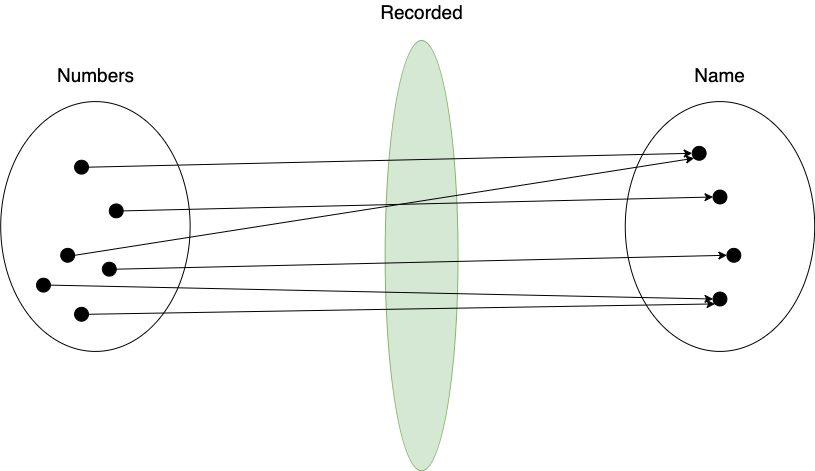
\includegraphics[scale=0.45]{images/Diagram.png}
        \caption{State of the System}
        \label{fig:Diagram}
        \end{figure}
    \item $numbers$ can be formally defined as: \\
    $\{ \forall x, y: numbers | (x \in numbers \wedge y \in numbers) \rightarrow x \neq y \}$
    \item
    \item
    \item As previously stated, the domain of \emph{recorded} is \emph{Numbers}. We know that \emph{Numbers} is the set 
    of all phone numbers recorded in contacts. Since not all elements of \emph{PhoneNumberType} are recorded, we can
    state that \emph{Numbers} is a subset of \emph{PhoneNumberType} as shown in the diagram displayed at \underline{question 1}.
    A partial function \emph{f} is a function that is defined for some subset \emph{A'} of \emph{A}, not forcing mapping for 
    all elements of set A such that $dom f \subset A$. Thus, \emph{recorded} is a partial function.
    \item We know that each element of \emph{Name} (the codomain) has to be associated with at least one element of 
    \emph{Numbers} (the domain). We also know that a name can be associated with multiple phone numbers. This type of 
    function is described as a surjective function. 
    \item The function \emph{recorded} can be formally defined as:\\
    $\{ \forall y \in \emph{Name},   \exists x \in \emph{Numbers} | recorded(x) = y \}$
\end{enumerate}

\newpage
\section{Problem 2: Class Contacts (35 pts)}

\subsection{Description:}
Define a formal specification in Object-Z for class \textit{Contacts} whose interface contains the
following \textit{robust specifications}:

\begin{itemize}
    \item \textbf{MakeNewContact}: Adds a new person to Contacts with a single phone number.
    \item \textbf{AddNumber}: Adds an additional phone number for an existing contact.
    \item \textbf{SearchForNumber}: : Returns a collection of phone numbers for a given person.
    \item \textbf{DeleteNumber}: Deletes an existing number.
\end{itemize}

\subsection{Answer:}

\begin{class}{Contacts}
\also
\upharpoonright (MakeNewContact, AddNumber, SearchForNumber, DeleteNumber) \\
\begin{state}
numbers: \mathbb{P}~PhoneNumberType\\
recorded : NameType \pfun PhoneNumberType\\
\where
numbers = dom~recorded
\end{state} \\
\begin{init}
recorded = \emptyset %\{ \}
\end{init} \\
\begin{op}{MakeNewContactOK}
\Delta (recorded) \\
number?: PhoneNumberType \\
name?: NameType \\
\ST
number? \notin numbers \\
name? \notin ran~recorded \\
recorded' = recorded \cup \{number? \mapsto name? \}
\end{op}\\
\begin{op}{AddNumberOK}
\Delta () \\
\ST
\end{op}\\
\begin{op}{SearchForNumberOK}
\Delta () \\
\ST
\end{op}\\
\begin{op}{DeleteNumberOK}
\Delta () \\
\ST
\end{op}\\
\begin{op}{Success}
response!: Message \\
\ST
response! = 'ok'
\end{op}\\
\begin{op}{NumberExists}
number?: PhoneNumberType \\
response!: Message \\
\ST
number? \in numbers \\
response! = 'Number~already~exists'
\end{op}\
\zbreak
\begin{op}{NameExists}
name?: NameType \\
response!: Message \\
\ST
name? \in ran~recorded \\
response! = 'Name~already~taken'
\end{op}\
\also
MakeNewContact \sdef (MakeNewContactOK \wedge Success) \oplus (NumberExists \lor NameExists) \\
AddNumber \sdef \\
SearchForNumber \sdef \\
DeleteNumber \sdef
\end{class}
\newpage
\section{Problem 3: Class Contacts2 (8 pts)}

\subsection{Description:}
Subclassify \textbf{Contacts} to introduce class \textbf{Contacts2} that behaves exactly like \textbf{Contacts},
while introducing a robust operation to search for a person, given a phone number through
operation \textbf{SearchForPerson}.

\subsection{Answer:}


\newpage

\section{Problem 4 (12 pts)}

\subsection{Description:}

Consider list $\Lambda = \langle w, x, y, z \rangle$, deployed to implement a Queue Abstract Data Type.

\begin{enumerate}

\item Let the head of $\Lambda$ correspond to the front position of the Queue. Implement operations \texttt{enqueue(el, $\Lambda$)} and \texttt{dequeue($\Lambda$)} using list construction operations. In both cases we can refer to $\Lambda'$ as the state of the list upon successful termination of one of its operations.

\item Let us now reverse the way we manipulate our data structure and let the head of $\Lambda$ correspond to the rear of the Queue.
\begin{enumerate}
\item What would be the result of $cons(el, \Lambda)$, and would it be a correct implementation for operation \texttt{enqueue(el, $\Lambda$)}?
\item What would be the result of $list(el, \Lambda)$, and would it be a correct implementation for operation \texttt{enqueue(el, $\Lambda$)}?
\item What would be the result of $concat(list(el), \Lambda)$, and would it be a correct implementation for operation \texttt{enqueue(el, $\Lambda$)}?
\end{enumerate}
\end{enumerate}


\subsection{Enqueue and dequeue operations with head of list as front of queue}

\subsubsection{enqueue(el, $\Lambda$)}
\begin{itemize}
    \item[] $\Lambda$' = concat($\Lambda$, list(el));
\end{itemize}

\subsubsection{dequeue($\Lambda$)}
\begin{itemize}
    \item element = head($\Lambda$);
    \item $\Lambda$' = tail($\Lambda$);
    \item[] where 'element' is the return value of the operation.
\end{itemize}



\subsection{Let head of A correspond to the rear of Queue}

\subsubsection{cons(el, $\Lambda$)}
\begin{enumerate}
    \item[] \textbf{Result:} $\langle el, w, x, y, z \rangle$
    \item[] It's the correct implementation for operation \texttt{enqueue(el $\Lambda$)} since it adds the new element to the rear of the queue (head of $\Lambda$). Hence, it is acceptable since it implements the Queue protocol.
\end{enumerate}

\subsubsection{list(el, $\Lambda$)}
\begin{enumerate}
    \item[] \textbf{Result:} $\langle el, \langle w, x, y, z \rangle \rangle$
    \item[] It's \textbf{not} the correct implementation for operation \texttt{enqueue(el $\Lambda$)} since it creates list containing A as a list inside. Hence, it is not acceptable because it does not implement the Queue protocol.
\end{enumerate}

\subsubsection{concat(list(el), $\Lambda$)}
\begin{enumerate}
    \item[] \textbf{Result:} $\langle el, w, x, y, z \rangle$
    \item[] It's the correct implementation for operation \texttt{enqueue(el $\Lambda$)} since it adds the new element to the rear of the queue (head of $\Lambda$). Hence, it is acceptable since it implements the Queue protocol.
\end{enumerate}

\newpage

\section{Problem 5 (12 pts)}
\subsection{Description:}

\noindent Let $A = \{ 0, 1, 2, 3, 4 \}$ and relations $R$, $S$, $T$, and $U$ on $A$ defined as follows:

\[ R = \{ (0, 0),  (0, 1),  (0, 3),  (1, 0),  (1, 1),  (2, 2),  (3, 0),  (3, 1), (3, 3), (4, 0), (4, 1), (4, 3), (4, 4)  \}\]

\[ S = \{ (0, 1),  (1, 1),  (2, 3),  (2, 4), (3, 0), (3, 4), (4, 0), (4, 1), (4, 4)  \}\]

\[ T = \{ (0, 3), (0, 4),  (2, 1), (3, 2), (4, 2), (4, 3) \}\]

\[ U = \{ (0, 0),  (0, 1), (0, 3), (1, 0), (1, 1), (1, 3), (2, 2), (3, 0), (3, 1), (3, 3), (4, 4) \}\]

\noindent Fill in the table below, using $\checkmark$, or $\times$.

\begin{center}
\begin{tabular}{|l|l|l|l|l|l|}
\hline
						&	&	$R$	&	$S$	&	$T$	& $U$\\
\hline
\textbf{Reflexive} 	&   &		&		&	&	 \\
\hline
\textbf{Irreflexive} 	&   &		&		&	&	 \\
\hline
\textbf{Symmetric} 	&   &		&		&	&	 \\
\hline
\textbf{Asymmetric} 	&   &		&		&	&	 \\
\hline
\textbf{Antisymmetric} &   &		&		&	&	 \\
\hline
\textbf{Transitive} 	&   &		&		&	&	 \\
\hline
\textbf{Equivalence} 	&   &		&		&	&	 \\
\hline
\textbf{Partial order} 	&   &		&		&	&	 \\
\hline
\end{tabular}
\end{center}

\subsection{Answer:}
\begin{center}
\begin{tabular}{|l|l|l|l|l|l|}
\hline
						&	&	$R$	&	$S$	&	$T$	& $U$\\
\hline
\textbf{Reflexive} 	    &   &$\checkmark$		&$\times$		&$\times$	&$\checkmark$	 \\
\hline
\textbf{Irreflexive} 	&   &$\times$		&$\times$		&$\checkmark$	&$\times$	 \\
\hline
\textbf{Symmetric} 	    &   &$\times$		&$\times$		&$\times$	&$\checkmark$	 \\
\hline
\textbf{Asymmetric} 	&   &$\times$		&$\times$		&$\checkmark$	&$\times$	 \\
\hline
\textbf{Antisymmetric}  &   &$\times$		&$\checkmark$		&$\checkmark$	&$\times$	 \\
\hline
\textbf{Transitive} 	&   &$\times$		&$\times$		&$\times$	&$\checkmark$	 \\
\hline
\textbf{Equivalence} 	&   &$\times$		&$\times$		&$\times$	&$\checkmark$	 \\
\hline
\textbf{Partial order} 	&   &$\times$		&$\times$		&$\times$	&$\times$	 \\
\hline
\end{tabular}
\end{center}

\underline{Relation R}
\begin{itemize}
    \item Reflexive:  Since (0,0), (1,1), (2,2) (3,3), (4,4) $\in R$, it is reflexive.
    \item Irreflexive: Not irreflexive since an element that is related to itself exists (i.e (0,0)).
    \item Symmetric: Not symmetric since (3,1) $\in R$, but (1,3) $\notin R$.
    \item Asymmetric: Not asymmetric since (0,1), (1,0) $\in R$.
    \item Antisymmetric: Not antisymmetric since (0,1), (1,0) $\in R$, but 0 $\neq$ 1.
    \item Transitive: Not transitive since (1,0), (0,3) $\in R$, but (1,3) $\notin R$. 
    \item Equivalence: Not an equivalence relation since it is not reflexive, symmetric and transitive.
    \item Partial order: Not a partial order relation since it is not reflexive, antisymmetric and transitive.
\end{itemize}


\underline{Relation S}
\begin{itemize}
    \item Reflexive: Not reflexive since (0,0) $\notin S$.
    \item Irreflexive: Not irreflexive since (1,1) $\in S$.
    \item Symmetric: Not symmetric since (0,1) $\in S$, but (1,0) $\notin S$.
    \item Asymmetric: Not asymmetric since (1,1) $\in S$, which is a self-loop.
    \item Antisymmetric: Since every element in $S$ is not bidirectional except for self-loops, it is antisymmetric.
    \item Transitive: Not transitive since (2,3), (3,0) $\in S$, but (2,0) $\notin S$.
    \item Equivalence: Not an equivalence relation since it is not reflexive, symmetric and transitive.
    \item Partial order: Not a partial order relation since it is not reflexive, antisymmetric and transitive.
\end{itemize}

\underline{Relation T}
\begin{itemize}
    \item Reflexive: Not reflexive since (0,0) $\notin S$.
    \item Irreflexive: Since no element that is related to itself belongs to $T$, it is irreflexive.
    \item Symmetric: Not symmetric since (0,3) $\in T$, but (3,0) $\notin T$.
    \item Asymmetric: Since no element in $T$ is bidirectional and there are no elements that are self-loops, it is asymmetric. 
    \item Antisymmetric: Since the relation is asymmetric, it is antisymmetric.
    \item Transitive: Not transitive since (0,3), (3,2) $\in S$, but (0,2) $\notin S$.
    \item Equivalence: Not an equivalence relation since it is not reflexive, symmetric and transitive.
    \item Partial order: Not a partial order relation since it is not reflexive, antisymmetric and transitive.
\end{itemize}

\underline{Relation U}
\begin{itemize}
    \item Reflexive: Since (0,0), (1,1), (2,2) (3,3), (4,4) $\in U$, it is reflexive.
    \item Irreflexive: Not irreflexive since an element that is related to itself exists (i.e (0,0)).
    \item Symmetric: Since every pair in $U$ is bidirectional, it is symmetric.
    \item Asymmetric: Not asymmetric since (0,1), (1,0) $\in U$.
    \item Antisymmetric: Not antisymmetric since (0,1), (1,0) $\in U$, but 0 $\neq$ 1.
    \item Transitive: Since $\forall a,b,c \in A$: ($aUb \wedge bUc$) $\rightarrow$ $aUc$, it is transitive.
    \item Equivalence: Since the relation is reflexive, symmetric and transitive, it is an equivalence relation.
    \item Partial order: Not a partial order relation since it is not reflexive, antisymmetric and transitive.
\end{itemize}

\newpage

\section{Problem 6 (8 pts)}
\subsection{Answer}

Consider the relation \textit{``is a subtype of''} as $R$ over the set $A = \{ rectangle, quadrilateral, square, \\parallelogram,rhombus\}$.
\\

$
R = \{(rectangle, quadrilateral), (rectangle, parallelogram), (square, rectangle),
\\(square, quadrilateral), (parallelogram, quadrilateral), (rhombus, quadrilateral),
\\(rhombus, parallelogram), (rectangle, rectangle), (quadrilateral, quadrilateral),
\\(square, square), (parallelogram, parallelogram), (rhombus, rhombus)\}
$
\\ \begin{enumerate}
    \item In order for a relation to be an equivalence relation, it must be reflexive, symmetric and transitive.
    \begin{itemize}
        \item $R$ is reflexive since every element in $A$ is related to itself. That is, $\forall a \in A: aRa$. 
        \item $R$ is not symmetric since $(rectangle, quadrilateral) \in R, but (quadrilateral, rectangle) \notin R.$
        \item $R$ is transitive since for elements $a, b, c$ in the set $A$, if $a$ and $b$ are related by $R$, and $b$ and $c$ are related by $R$, then $a$ and $c$ are also related by $R$. That is, $\forall a,b,c \in A: (aRb \wedge bRc) \rightarrow aRc$.
    \end{itemize}
    Since the relation is reflexive, transitive, but not symmetric, it is not an equivalence relation.
    
    \item In order for a relation to be a partial order relation, it must be reflexive, antisymmetric and transitive.
    \begin{itemize}
        \item R is antisymmetric since for elements $a, b$ in the set $A$, if $aRb$ and $bRa$, then $a=b$. In other words, there is no pair in R such that the reverse of this pair exists, unless the pair contains identical elements.
    \end{itemize}
    From the previous point, it has been concluded that $R$ is reflexive and transitive. Since $R$ is also antisymmetric, it is a partial order.
    \\
    \\
    The Hasse diagram of $R$ is shown in the following figure:
    \newpage
    \begin{figure}[h]
        \centering
        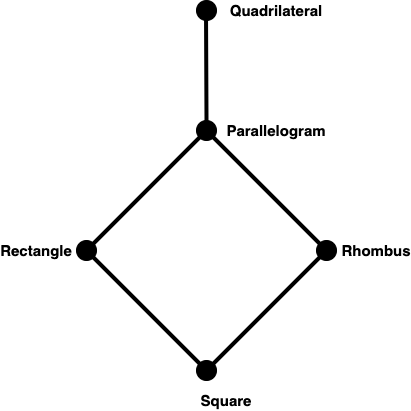
\includegraphics[scale=0.5]{Hasse}
        \caption{Hasse Diagram for Problem 6}
        \label{fig:Hasse}
    \end{figure}
    From figure \ref{fig:Hasse}, it can be concluded that the maximal element is $Quadrilateral$, since it does not have any successors, and the minimal element is $Square$, since it does not have any predecessors.
    
\end{enumerate}
\newpage

\section{Problem 7 (8 pts)}
\subsection{Description}

Consider the set $A = \{ w, x, y, z \}$, and the relations

\begin{description}

\item $S = \{ (w, x), (w, y), (x, w), (x, x), (z, x) \}$

\item $T = \{ (w, w), (w, y), (x, w), (x, x),  (x, z), (y, w), (y, y), (y, z) \}$
\end{description}

\noindent Find the following compositions:

\begin{enumerate}
\item $S \circ T$

\item $T \circ S$

\item $T^{-1} \circ S^{-1}$
\end{enumerate}

\noindent \textbf{NOTE}: Some authors (e.g. Rosen) adopt a different ordering of operands than the one we use in our lecture notes. Please follow the ordering (and the definition) of the lecture notes.\\

\subsection{Answer}

\begin{enumerate}
    \item $S \circ T = \{ (w, w), (w, x), (w, z), (w, y), (x, w), (x, y), (x, x), (x, z),(z, w), (z, x), (z, z) \}$
    
    \item $T \circ S = \{ (w, x), (w, y), (x, x), (x, y), (x, w), (y, y), (y, x)  \}$
    
    \item $T^{-1} \circ S^{-1} = \{ (w, x), (w, w), (w, z), (x, w), (x, x), (x, z), (y, x),(y, w), (z, w), (z, x), (z, z) \}$
\end{enumerate}

\newpage


\section{Problem 8 (12 pts)}
\subsection{Description}

Consider sets $A = \{1, 2, 3, 4, 5, 6 \}$ and $B = \{ a, b, c, d, e, f \}$.

\begin{enumerate}

\item Determine the type of the correspondence in each of the following cases, or indicate if the correspondence is not a function.

\begin{enumerate}
\item $\{ 1 \mapsto b, 2 \mapsto c, 3 \mapsto e, 4 \mapsto d, 5 \mapsto f, 3 \mapsto a \}$

\item $\{ 1 \mapsto a, 2 \mapsto d, 3 \mapsto a, 4 \mapsto f, 5 \mapsto d, 6 \mapsto c \}$

\item $\{ 1 \mapsto c, 2 \mapsto b, 3 \mapsto d, 4 \mapsto e, 5 \mapsto e, 6 \mapsto f  \}$

\item $\{ 1 \mapsto b, 2 \mapsto c, 3 \mapsto e, 4 \mapsto d, 5 \mapsto f, 6 \mapsto a \}$
\end{enumerate}

\noindent Fill in the table below, using $\checkmark$, or $\times$.

\begin{center}
\begin{tabular}{|l|c|c|c|c|c|}
\hline
		& Inective		& Surjective	& Bijective 	& \multicolumn{1}{m{3cm}|}{Neither injective nor surjective}	&	Not a function	\\
\hline
(a)		& 		& 		& 	& 			&$\checkmark$  \\
\hline

(b)		& 		& 		& 		& $\checkmark$	&	 \\
\hline


(c)		& 		& 		& 	& $\checkmark$	&  \\
\hline

(d)		& 		& 		&$\checkmark$ 		&	&  \\
\hline
\end{tabular}
\end{center}


\item Is it possible to construct a function $f : A \rightarrow B$ which is surjective and not injective?  Discuss.
\end{enumerate}

\subsection{Answer}

\begin{enumerate}
	\item See table above
	\item A function from $A$ to $B$ is an assisgnment of each element of the domain to exactly one element of the codomain.
	We know that a function is surjective if each of the elements of the codomain is mapped by at least one element of the domain.
	\\
	Therefore, if a function $f : A \rightarrow B$ is to be surjective, all elements of $A$ must point to one and only one 
	element of $B$ (definition of a function) and all elements of $B$ must be pointed by at least one element of $A$ (definition
	of a surjective function).
	\\
	Fianlly, we know that $A$ and $B$ have the same cardinality, namely 6. This yields that for $f$ to be surjective, all elements
	of $B$ have to be pointed by exactly one element of $A$, making $f$ an injective function. 
	\\
	In conclusion, given sets $A$ and $B$, it is impossible for a function $f : A \rightarrow B$ to be surjective without
	being injective.  
\end{enumerate}

\newpage

\section{Problem 9 (20 pts)}
\subsection{Description}

\noindent Consider the following relation:

\[ laptops : Model \leftrightarrow Brand \]

\noindent where

\[
laptops = \\
\hspace{5mm} \{ \\
\hspace{10mm} legion5 \mapsto lenovo,\\
\hspace{10mm} macbookair \mapsto apple,\\
\hspace{10mm} xps15 \mapsto dell,\\
\hspace{10mm} spectre \mapsto hp,\\
\hspace{10mm} xps13 \mapsto dell,\\
\hspace{10mm} swift3 \mapsto acer,\\
\hspace{10mm} macbookpro \mapsto apple,\\
\hspace{10mm} dragonfly \mapsto hp,\\
\hspace{10mm} envyx360 \mapsto hp\\
\hspace{5mm} \}
\]

\begin{enumerate}

\item What is the domain and the range of the relation?\\

\item What is the result of the expression

\[ \{ xps15, xps13, swift3, envyx360 \}  \lhd laptops \]

\noindent What is the meaning of operator $\lhd$ and where would you deploy such operator in the context of a database management system?

\item What is the result of the expression

\[ laptops \rhd \{ lenovo, hp \} \]

\noindent What is the meaning of operator $\rhd$ and where would you deploy such operator in the context of a database management system?

\item What is the result of the expression

\[ \{ legion5, xps15, xps13, dragonfly \} \ndres laptops \]

\noindent What is the meaning of operator $\ndres$ and where would you deploy such operator in the context of a database management system?

\item What is the result of the expression

\[ laptops \nrres \{ apple, dell, hp \} \]

\noindent What is the meaning of operator $\nrres$ and where would you deploy such operator in the context of a database management system?

\item Consider the following expression

\[ laptops \oplus \{ ideapad \mapsto lenovo \} \]

\begin{enumerate}
\item What is the result of the expression?

\item What is the meaning of operator $\oplus$ and where would you deploy such operator in the context of a database management system?

\item Does the result of the expression have a permanent effect on the database (relation)? If not, describe in detail how would you ensure a permanent effect. 

\end{enumerate}

\end{enumerate}


\subsection{Answer}
\begin{enumerate}

\item dom laptops = \{legion5, macbookair, xps15, spectre, xps13, swift3, macbookpro, dragonfly, envyx360 \}
\\ \\
ran laptops = \{lenovo, apple, dell, hp, acer\} \\

\item \{ xps15, xps13, swift3, envyx360 \}  $\lhd$ laptops  = \\
\{ xps15 $\mapsto$ dell, \\
xps13 $\mapsto$ dell, \\
swift3 $\mapsto$ acer, \\
envyx360 $\mapsto$ hp \}
\\ \\
$\lhd$ is a domain restriction operator that selects pairs from the database table (in this case from laptops database table) based on the first element. Such operator is deployed in the database management system for query operation. It is specifically a select query (a data retrieval query).\\
 
\item laptops $\rhd$ \{ lenovo, hp \} = \\
\{legion5 $\mapsto$ lenovo, \\
spectre $\mapsto$ hp, \\
dragonfly $\mapsto$ hp, \\
envyx360 $\mapsto$ hp \}
\\ \\
$\rhd$ is a range restriction operator that selects pairs from the database table (in this case from laptops database table) based on the second element. As previously mentioned, this is also deployed in database management for query operation (specifically a select query used for data retrieval query). \\

\item \{ legion5, xps15, xps13, dragonfly \} $\ndres$  laptops = \\
\{macbookair $\mapsto$ apple, \\
spectre $\mapsto$ hp, \\
swift3 $\mapsto$ acer, \\
macbookpro $\mapsto$ apple, \\
envyx360 $\mapsto$ hp \}
\\ \\
$\ndres$ is a domain subtraction operator that removes all pairs based on the first element (the domain of the element). In other words, it removes all pairs where model is anything specified within the brackets. This is also a query operation (more specifically an action query) where additional operation (such as a deletion in this case) is applied on  the data.\\

\item laptops $\nrres$ \{ apple, dell, hp \} = \\
\{legion5 $\mapsto$ lenovo, \\
swift3 $\mapsto$ acer \}
\\ \\
$\nrres$ is a range subtraction operator that removes all pairs based on the second element (the range of the relation). In other words, it removes all pairs where the brand is anything specified within the brackets. This is an action query, where a deletion (in this case) is applied on the data.\\

\item 
\begin {enumerate} 
\item laptops $\oplus$ \{ ideapad $\mapsto$ lenovo \} = \\
\{ legion5 $\mapsto$ lenovo, \\
macbookair $\mapsto$ apple, \\
xps15 $\mapsto$ dell, \\
spectre $\mapsto$ hp, \\
xps13 $\mapsto$ dell, \\
swift3 $\mapsto$ acer, \\
macbookpro $\mapsto$ apple, \\
dragonfly $\mapsto$ hp, \\
envyx360 $\mapsto$ hp, \\
ideapad $\mapsto$ lenovo\} \\

\item $\oplus$ is an insertion operator used in model database updates for relational overriding. Therefore, the specified element within the bracket is added to the already existing laptop set. Such operator is deployed in the database management system for query operation, specifically an action query, where (in this case) the action is an insertion of data to the existing database.  \\

\item The result will not have a permanent effect on the database, because this is just an  evaluation of the expression. To ensure a permanent effect, the result of this expression must be assigned to a variable (laptops') which will hold the state of the set upon successful evaluation of the right-hand side expression: \\
laptops' = laptops $\oplus$ \{ ideapad $\mapsto$ lenovo \}
\end{enumerate}

\end{enumerate}



\end{document}
